\chapter{Background}
This thesis is based on several kinds of research of auto-tuning, evolutionary algorithms, and software optimization. This chapter summarizes the important aspects and details of approaches and optimization techniques used in the succeeding chapters.  

\section{Multi-Quality Auto-Tuning~(MQuAT)}

Multi-Quality Auto-Tuning (MQuAT) – is an approach to self-adaptive software, which provides design and operation principles for software systems that automatically provide the best possible utility to the user while producing the least possible cost.
It is based on the design-time part, which represents a new development method for self-optimizing systems and runtime parts, which concerns operation principles, namely,  novel techniques to runtime self-optimization~\cite{gotz13}.

\subsection{Design principles of MQuAT}

MQuAT presented a new method of developing self-optimized software. In which software is proposed to be constructed from components with specifically defined limits. In addition, components are intended to comprise multiple implementations, each providing the same but differing functionality in their non-functional behavior. Therefore, the design principle is the critical factor for runtime optimization because when there is a different configuration, optimization can be done, and the optimal or almost optimal configuration can be selected. To compare different implementations of the software component, they need to be specified with their non-functional properties (NFP)~\cite{gotz13}.
A new meta-architecture of the self-optimizing software system was created To highlight this fundamental principle. It called the cool component model~\cite{gotz10}.
A specialty of MQuAT is the application of QoS contracts to cover non-functional implementation behavior as well as the interrelationships of different components between NFPs. Contracts naturally describe the relationship between provisions and requirements.

\subsection{Operation principles of MQuAT}

The core runtime approach proposed in MQuAT is the THE Auto-Tuning Runtime Environment (THEATRE)\cite{gotz10, gotz12}.
The concept of runtime environment contains three layers: a user, software, and a resource layer. All of them depicted in Figure ~\ref{fig:threelayersmquat}

\begin{figure}
	\centering
	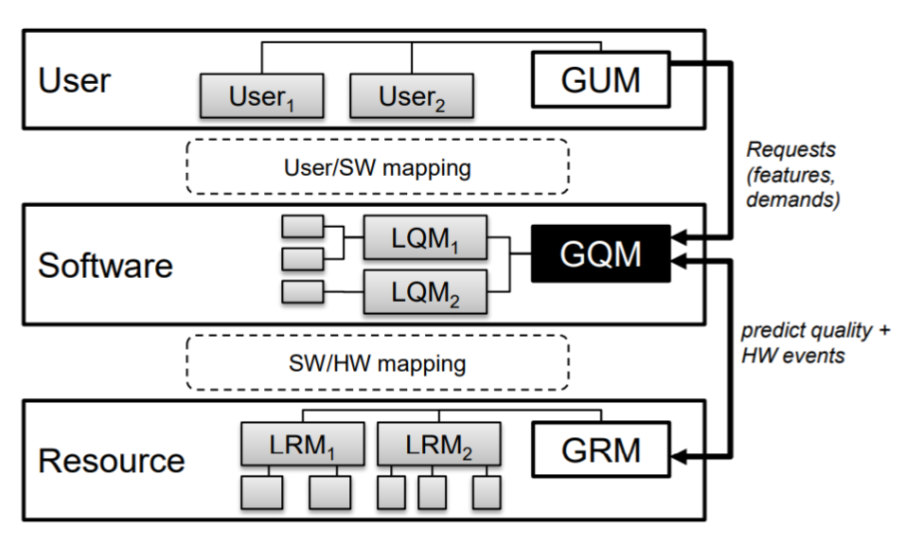
\includegraphics[width=\textwidth]{images/ThreeLayersMQuAT}
	\caption[Three layers of MQuAT]{Three layers of MQuAT}
	\label{fig:threelayersmquat}
\end{figure}

The user layer invokes features and identifies their specifications. The  Global  User  Manager  (GUM)  is required to manage the mapping between users and software component implementations and to coordinate the requests. User requests are minimal software system specifications that have to be met to satisfy the user. The general aim of the runtime system is to help the user as effectively as possible about the purposes of the user~\cite{gotz13}.

The software layer contains all software components, and it's implementations. Each component has a Local Quality Manager(LQM), which responsible for controlling the set of components~\cite{gotz13, ahmad18}. Also, there is a single Global Quality Manager (GQM) which carry out the study and preparation phases of the feedback loop, while the LQM is responsible for the implementation process~\cite{gotz13}.

The resources layer comprises physical (e.g., CPU or RAM) as well as virtual resources(e.g., operating system).
To controlling and monitoring all resources, the Global Resource Manager(GRM) is presented. Each resource has its own Local Resource Manager (LRM), which has in-depth knowledge about its resource and the ability to steer the resource by~\cite{gotz13, ahmad18}.

\subsection{MQuAT combine the design time and runtime}

\begin{figure}
	\centering
	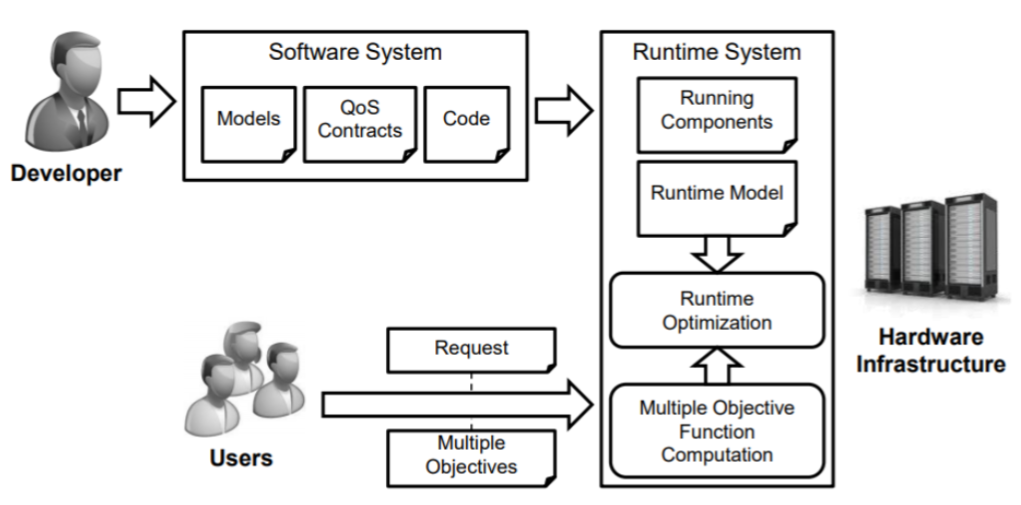
\includegraphics[width=\textwidth]{images/CombinedMQuAT}
	\caption[Combined structure of MQuAT]{Combined structure of MQuAT}
	\label{fig:CombinedMQuAT}
\end{figure}

As showed in Figure ~\ref{fig:CombinedMQuAT}, in addition to the actual code, the developer is creating the models and quality contracts. The users interact with the system at runtime and prepare their objectives and requests. 
In addition to the running components, the runtime system includes a runtime model, representing the current state of the system. The objectives of the user are transformed into objective functions of an optimization program prior to optimization. Depending on the type of optimization technique used, either all users ' objectives are merged into a single objective function, or one objective function is extracted per purpose. Such objective functions and the system's runtime model are used by the runtime optimization method to produce formulations of the optimization problem for the respective technique. Finally, the system determines whether the optimal configuration differs from the actual configuration~\cite{gotz13, ahmad18}.

For more details about MQuAT, please read refer~\cite{gotz13}. For this thesis, we are discussing a solver of the MQuAT problem that is based on MQuAT. Hence, detailed knowledge about MQuAT is not required. 


\section{MQuAT problem}

MQuAT problem was presented in ~\cite{gotz18}, and it consists of two problems:

\begin{itemize}
	\item Resource allocation in which the mapping of software component implementation to hardware resource leads to the least cost
	\item Variant selection, which provides the best utility by selecting better software implementations.
\end{itemize} 

To solve this problem was presented new generic metamodel. Both problems are interrelated by user requests specifying minimum requirements on the provided non-functional properties (i.e., minimum utility) while searching for a selection and mapping both to maximize utility and minimize costs. Correctness denotes that only solutions that \textit{do not violate} the users minimum requirements are considered \textbf{valid}.

The problem to be solved is selecting variants of software components and mapping them based on user requests to suitable hardware resources.

The MQuAT problem could be described as a metamodel which consists of:
\paragraph{Hardware metamodel}, which consists of hierarchically structured resource types and resources as instances of these types. So the hardware model composes static awareness of resources (types) and knowledge of runtime (instances). Certain types of resources can run the software, i.e., they are valid targets for software implementation mapping. The container attribute is used to mark such types. Figure~\ref{fig:HWmodel} depicted Hardware metamodel.

\begin{figure}
	\centering
	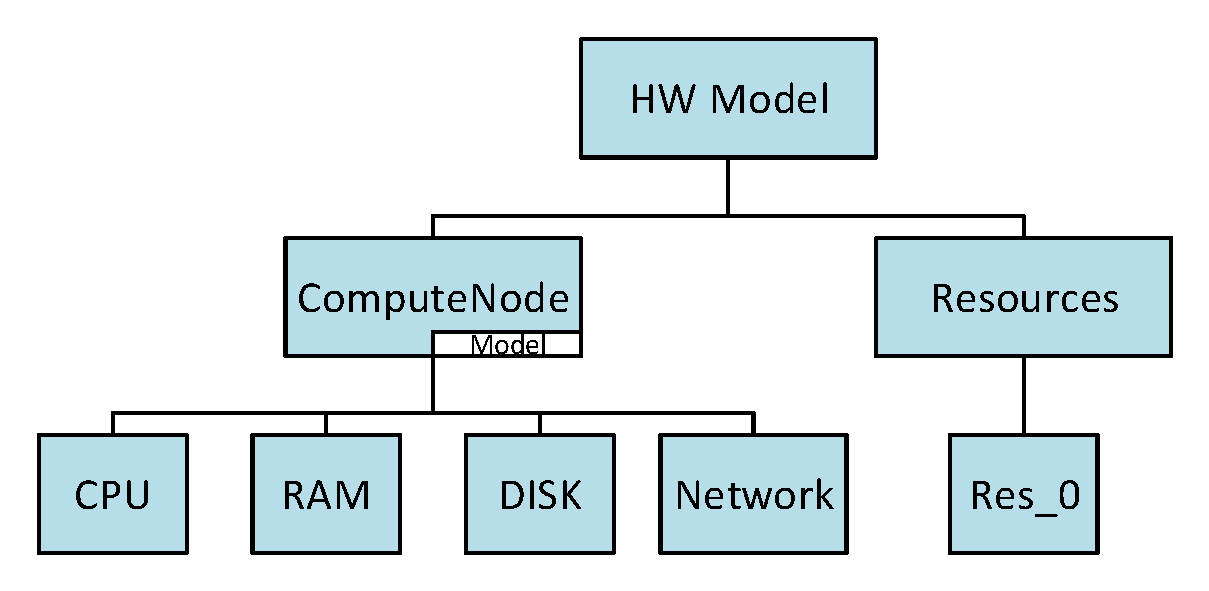
\includegraphics[width=\textwidth]{images/HWModel}
	\caption[Hardware meta-model]{Hardware meta-model}
	\label{fig:HWmodel}
\end{figure}


In addition, a set of properties further characterize resource types. Resources specify then specific values for these properties. As an example, the resource type RAM could be defined with a property amount of memory and marked as a container

\paragraph{Software metamodel} showed on Figure~\ref{fig:SWModel}. Its main element called component and represents some functionality.
Each component consists of implementations that provide this functionality, requiring additional components or resources to complete their work. 

\begin{figure}
	\centering
	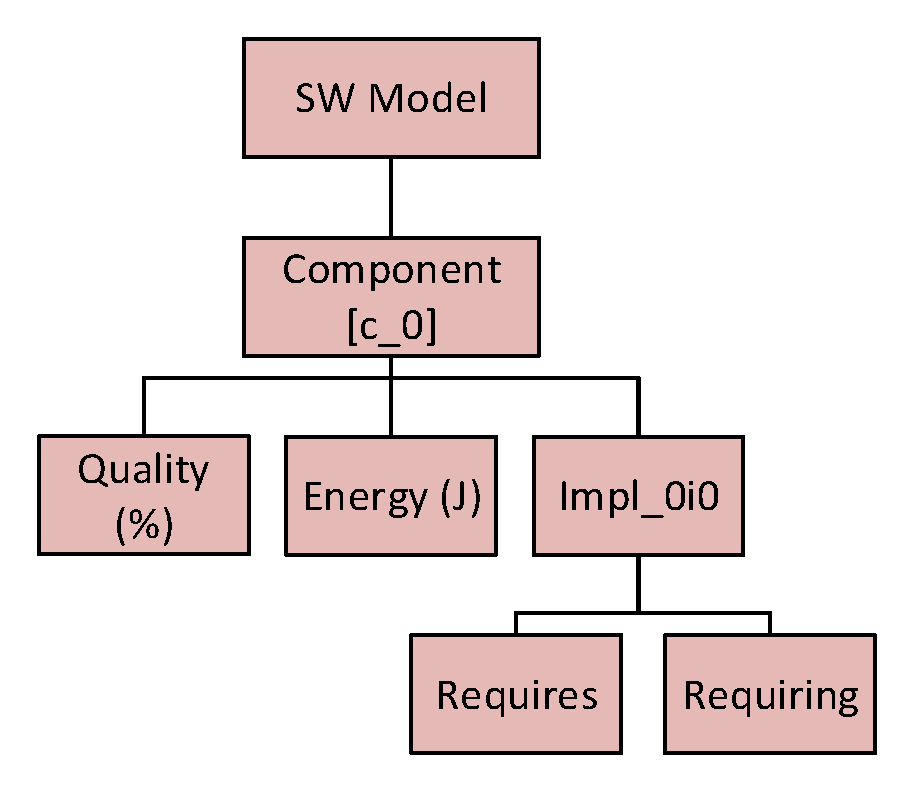
\includegraphics[width=0.75\textwidth]{images/SWModel}
	\caption[Software meta-model]{Software meta-model}
	\label{fig:SWModel}
\end{figure}

\paragraph{The Objective} specifies how to calculate a solution's objective value, i.e., for which value(s) the problem should be optimized. This selects a property to optimize for, and an objective function to define how to aggregate all values of this property.

\paragraph{A Request} represents a user requirement, which specifies which algorithm should be used to execute parameters and requirements. Requests contain their functional requirements by referring to a target software component, limitations on non-functional requirements (e.g., quality).\\

Full problem depicted on Figure~\ref{fig:mquatmodel}

\begin{figure}
	\centering
	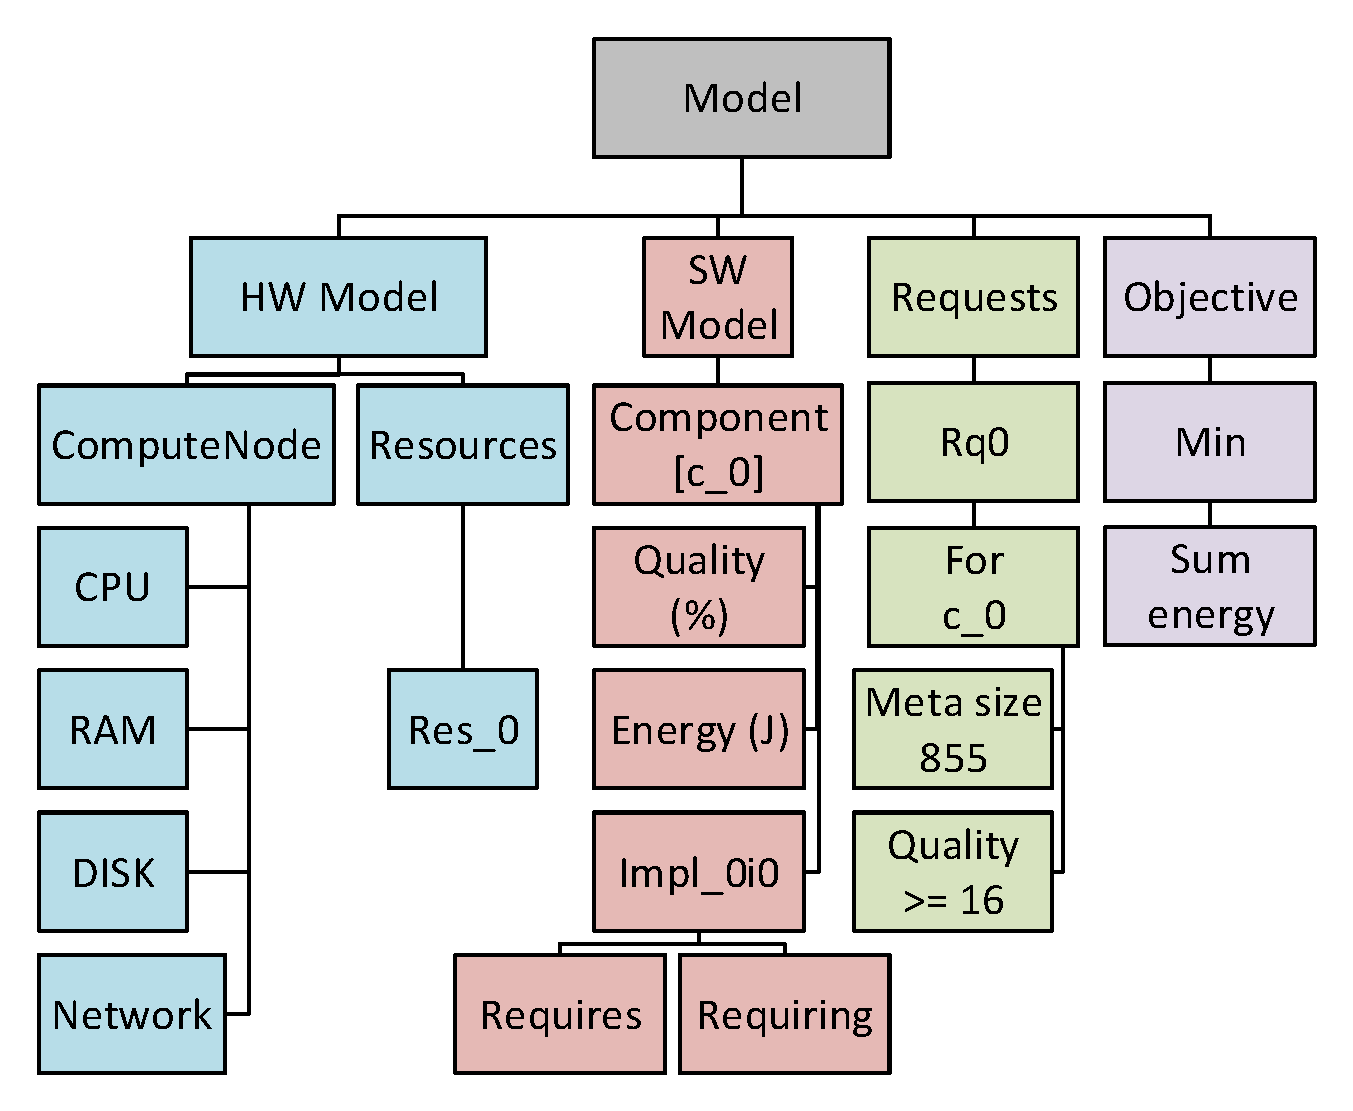
\includegraphics[width=\textwidth]{images/MQuATModel}
	\caption[MQuAT problem model]{MQuAT problem model}
	\label{fig:mquatmodel}
\end{figure}

There are some constraints that are grouped in Architectural, Request, and Negotiation constraints groups.

\begin{itemize}
	\item Architectural constraints ensure that each request is fulfilled, selecting exactly one implementation per component and deploying no more than one implementation on one resource.
	\item Request constraints ensure components are selected for each request so as to provide the requested non-functional properties.
	\item Negotiation constraints ensure non-functional requirements are met depending on the implementation.
\end{itemize}

There are additional constraints due to problem generation:

\begin{itemize}
	\item structures for the software and hardware components are fixed to ensure comparability,
	\item computeNode that represents a regular computer hardware consist of one or more CPUs, RAM memory, disk, and a networking interface,
	\item software model has a simple tree structure,
	\item fixed branching factor of two.
\end{itemize}

Each MQuAT problem is characterize by four parameters:

\begin{itemize}
	\item[variants] - the number of implementations for each software component,
	\item[requests] - the number of requests to run software components, that described by user, 
	\item[depth] - depth of the software tree, that describes dependency of software components,
	\item[resources] - resource ratio of the minimally required resources.
\end{itemize}

\section{The solution of the MQuAT problem}

The solution is computed by the MQuAT solver. There are many solvers:

\begin{itemize}
	\item Simple solver, which goes step by step from one solution candidate to another.
	\item ILP solver, which generates integer linear programming (ILP) problem from the MQUAT problem and after that solve it.
	\item Random solver - tries random solution candidates.
	\item Simulated Annealing (SA) solver, based on the simulated annealing meta-heuristic~{pukhkaiev19}.
	\item Genetic solver that uses a genetic algorithm to solve the problem.
\end{itemize}

In this thesis, we talk about Genetic solver in detail in the next sections.
The solution could be represented as a tree structure. An example of the solution shown in Figure ~\ref{fig:SolutionModel}

It contains a list of assignments. Each assignment select one implementation of required component and map it to the resources~\cite{gotz18}.
A solution is valid if for each user request

\begin{enumerate}
	\item an implementation is deployed for the target component,
	\item for each component required implementation is deployed,
	\item all necessary (non-functional) property clauses (including request constraints) are met,
	\item at most one implementation for each resource is deployed.
\end{enumerate}

If it is valid and no other solution has a better objective value, then a solution is optimal~\cite{gotz18}.

\section{Genetic algorithm}
\label{sec:GeneticAlgorithm}

Evolutionary algorithms are a subset of evolutionary computation and belong to set of modern heuristics-based search method.~\cite{vikhar16}
Appeared as a result of the influence of the biological evolution on computer scientists. This domain contains different types.
There are

\begin{itemize}
	\item Genetic algorithm 
	\item Genetic programming
	\item Evolutionary programming
	\item Evolution strategy
\end{itemize}

\begin{figure}
	\centering
	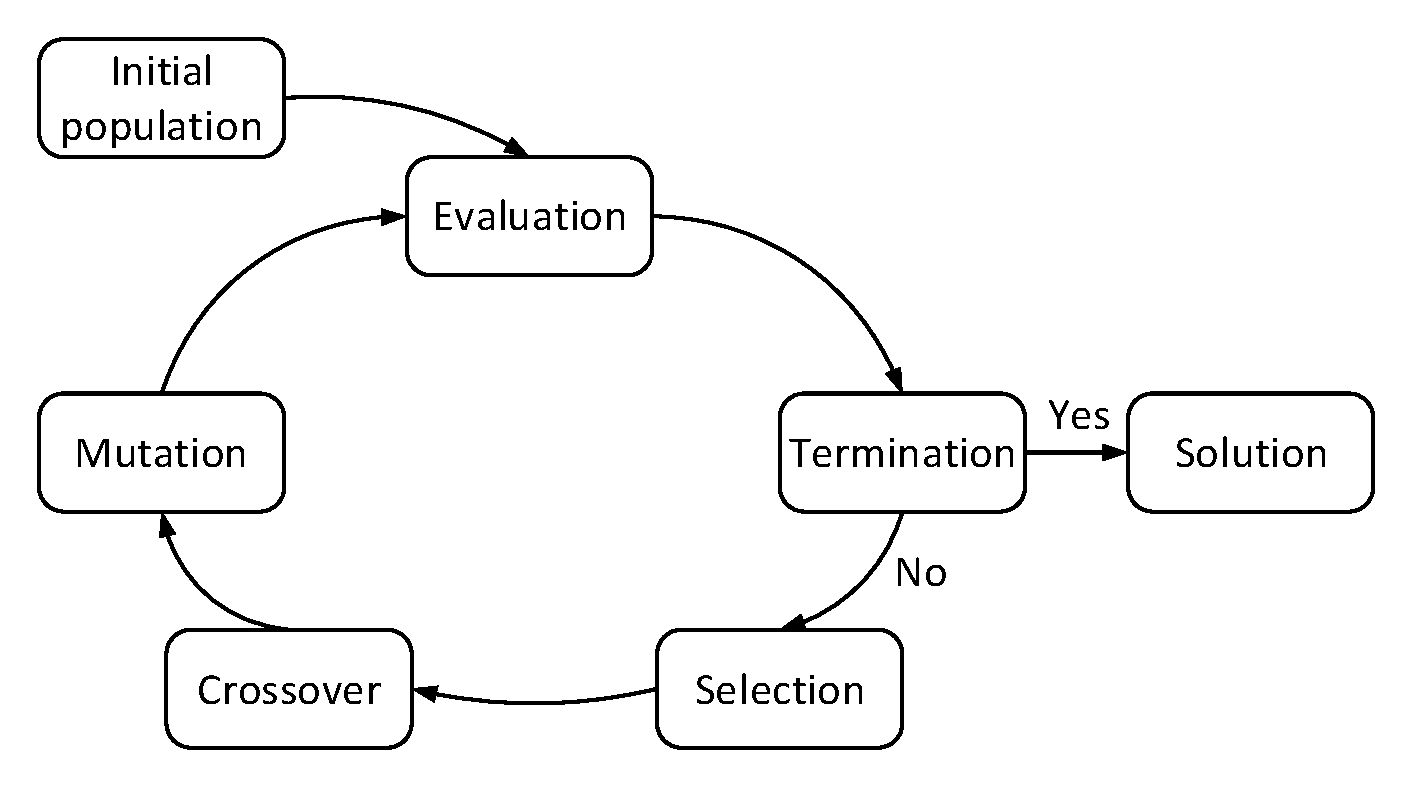
\includegraphics[width=0.8\textwidth]{images/GeneticLoop}
	\caption[Main loop of the genetic algorithm]{Main loop of the genetic algorithm}
	\label{fig:GeneticLoop}
\end{figure}

Main principle of GA looks like a loop with several steps.
The first step is the creation of an initial population - a set of randomly created individuals; each of them represents one solution. 
The second step is Evaluation. Calculate the fitness or objective function of the current population.
If the solution is founded and all requirements for the termination are fulfilled, then we get the final solution. Otherwise, select the best candidates to create a new generation.
In step 4, using recombination and mutation on selected candidates, GA creates a new generation of the population. And after that, evaluate it.

GA based on different components and operators.

\subsection{Selector}\label{sec:GeneticAlgorithm:Selector}

The selector is one of the most important components of GA. It selects \textit{\textbf{mu}} number of individuals from the population, that used to create new \textit{\textbf{lambda}} number of individuals.

There are many different selection algorithms

\begin{itemize}
	\item NSGA2 (Non-dominated sorting based genetic algorithm)
	\item SPEA2 (Strength Pareto Evolutionary Algorithm)
	\item NSGA3\todo{litref}
	\item SPEA3\todo{litref}
	\item PDE \todo{litref}
\end{itemize}

In this thesis, we focus on a selection algorithm only as a parameter of a genetic algorithm and use NSGA2 and SPEA2 due to software constraints of the used framework. 
\todo{Will add more information about selectors}

\subsection{crossover}\label{sec:GeneticAlgorithmCrossover}

Crossover is an operator of a genetic algorithm that allows the recombination of two individuals by swapping some genes between them.
In general, the crossover has several parameters such as

\begin{itemize}
	\item Crossover rate - parameter that describes the probability of two chromosomes to exchange their genes.
	\item Crossover point - the point in which the exchange could be done.
\end{itemize}

The principle of the crossover is next.
Firstly, select the crossover point. For example, a chromosome could be described as a vector of bits. Then the crossover point is the start index of bits, which were replaced by another chromosome.
Secondly, swap genes between chromosomes.

\begin{figure}
	\centering
	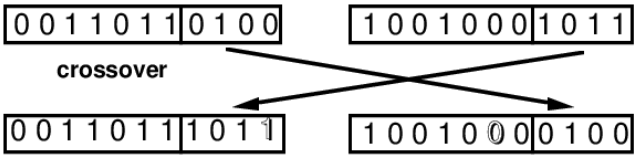
\includegraphics[width=0.5\textwidth]{images/crossoverVector.png}
	\caption[Example of the crossover]{Example of the crossover between chromosome that described as a vector of bits}
	\label{fig:crossoverVector}
\end{figure}

\subsection{mutation}\label{sec:GeneticAlgorithmMutation}

The mutation is an operator of a genetic algorithm that changes a single gene in a chromosome. As a crossover operator, a mutation has parameters:

\begin{itemize}
	\item Mutation rate - parameter that describes the probability of mutation.
\end{itemize}

To perform a mutation on chromosome need to do:

\begin{enumerate}
	\item Randomly select gene which mutates
	\item Change selected gene to another.
\end{enumerate}

\begin{figure}
	\centering
	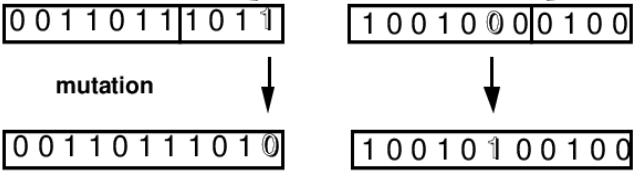
\includegraphics[width=0.5\textwidth]{images/MutationVector.png}
	\caption[Example of the mutation]{Example of the mutation between chromosome that described as a vector of bits}
	\label{fig:MutationVector}
\end{figure}

Figure~\ref{fig:MutationVector} presented a simple mutation on the chromosome that described as a vector of bits.




\section{Genetic solver}\label{sec:GeneticSolver}
To solve the MQuAT problem using a genetic algorithm, the genetic solver was developed by Jamal Ahmad in ~\cite{ahmad18}. And further improved by Johannes Mey.

This solver is based on Opt4J framework~\footnote{http://opt4j.sourceforge.net/download.html}. It's an open-source framework that gives the opportunity to implement a genetic algorithm for custom optimization problem by specifying several modules and classes.

To solve the custom problem using genetic algorithm, the user needs to create several things:

\begin{enumerate}
	\item Creator is needed to create a random genotype for the initial population.
	In the genetic solver Creator create the genotype by creating a random solution model and transform it into a Tree Shape Genotype structure.
	\item Decoder is needed to perform decoding the tree shape genotype into phenotype. The phenotype, in this case, is a Solution Model of MQuAT.
	\item Evaluator calculates the objective functions of the solution. In the case of genetic solver, the Evaluator calculates two objectives: 
	
	\begin{itemize}
		\item Validity errors - number of violated contracts
		\item Energy value - energy consumption
	\end{itemize}

\end{enumerate}

If your genotype can't be described as a vector, then you first need to implement:

\begin{enumerate}
	\item Genotype
	\item Crossover operator
	\item Mutation operator
\end{enumerate}

\subsection{Tree Shape Genotype}

Because of the problem model of MQuAT, which requires mapping of implementations to resources, in genetic solver was created Tree Shape Genotype~\cite{ahmad18}.
The example of this genotype shown on Figure~\ref{fig:TreeShapeGenotypeExample}

\begin{figure}
	\centering
	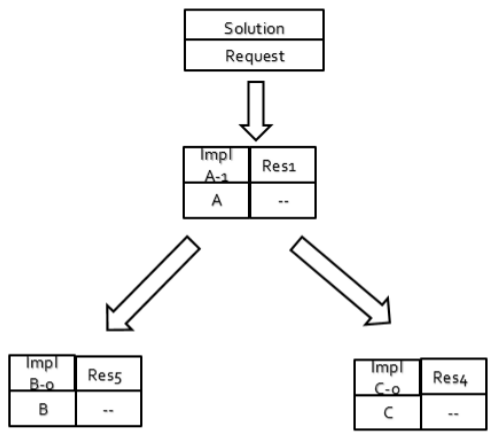
\includegraphics[width=0.6\textwidth]{images/TreeShapeGenotypeExample.png}
	\caption[Example of the Tree Shape Genotype]{Example of the Tree Shape Genotype}
	\label{fig:TreeShapeGenotypeExample}
\end{figure}

The first node in this genotype contains the input request. The second node represents the mapping of the user component. In this node, Impl A-1 is selected rather than Impl A-0 of the user component. As shown in Figure~\ref{fig:TreeShapeGenotypeExample}, this implementation is mapped to Hardware-Resources1. Moreover, Impl A-1 also requires software components B and C that have only one Impl B-0 and Impl C-0 implementation and are mapped to Hardware-Resource5 and Hardware-Resource4, respectively.

\subsection{Crossover operator}

This operator performs a crossover between two Tree Shaped Genotypes and are performed on software implementation and hardware resource in each tree shape genotype. Figure~\ref{fig:GeneticSolverCrossover} depicted the crossover. 
During this process, there is a check that ensures that the implementation and resources are not the same. If this check showed that comparing nodes are the same, then crossover goes recursively to child nodes and performs the check.
If the check showed that nodes are not the same, they swap the implementation, the resource, and all lower substructure.

\begin{figure}
	\centering
	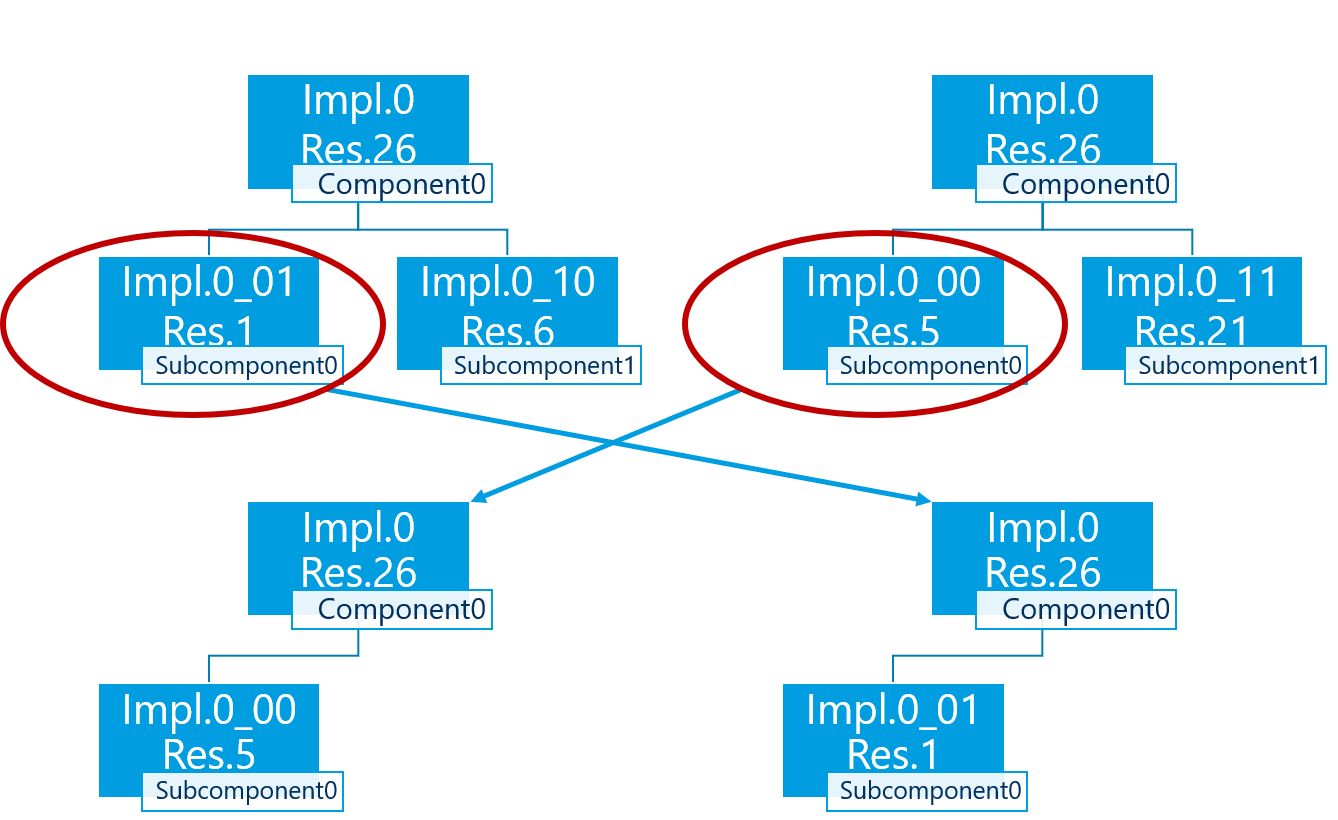
\includegraphics[width=0.9\textwidth]{images/GeneticSolverCrossover.png}
	\caption[Crossover in Tree Shape Genotype]{Example of crossover between two Tree Shape Genotypes}
	\label{fig:GeneticSolverCrossover}
\end{figure}



\subsection{Mutation operator}

Mutation operation is used to randomly add new features to the tree-shaped genotype. Figure~\ref{fig:GeneticSolverCrossover} depicts the mutation process in which with some probability to mutate current node or recursively go down to children.
There are two more probabilities that represent a chance of mutation in implementation and resource accordingly. 

\begin{figure}
	\centering
	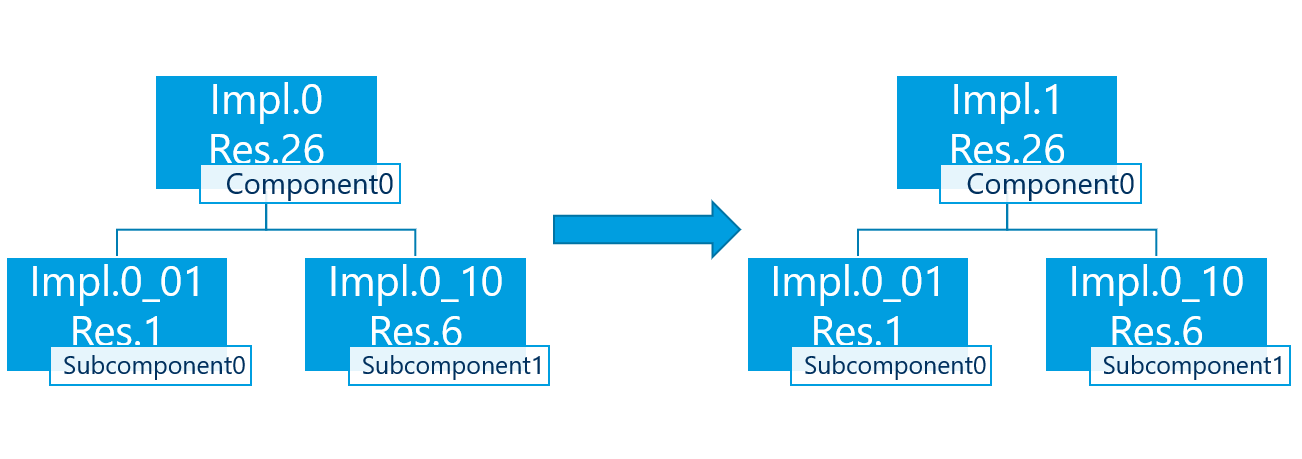
\includegraphics[width=\textwidth]{images/GeneticSolverMutation.png}
	\caption[Mutation in Tree Shape Genotype]{Example of mutation between two Tree Shape Genotypes}
	\label{fig:GeneticSolverMutation}
\end{figure}

\section{Parameter Tuning Strategies for GA}\label{sec:Parameter Tuning Strategies}

information from literature!\todo{will add more in next draft}

\section{BRISE}

BRISE is a software product line (SPL) for parameter tuning~\cite{pukhkaiev19}.
This SPL has two conceptual parts:

\begin{itemize}
	\item Static part describes the main flow of parameter tuning, task management, and reporting.
	\item Configurable part should be configured for each experiment.
\end{itemize}

\begin{figure}
	\centering
	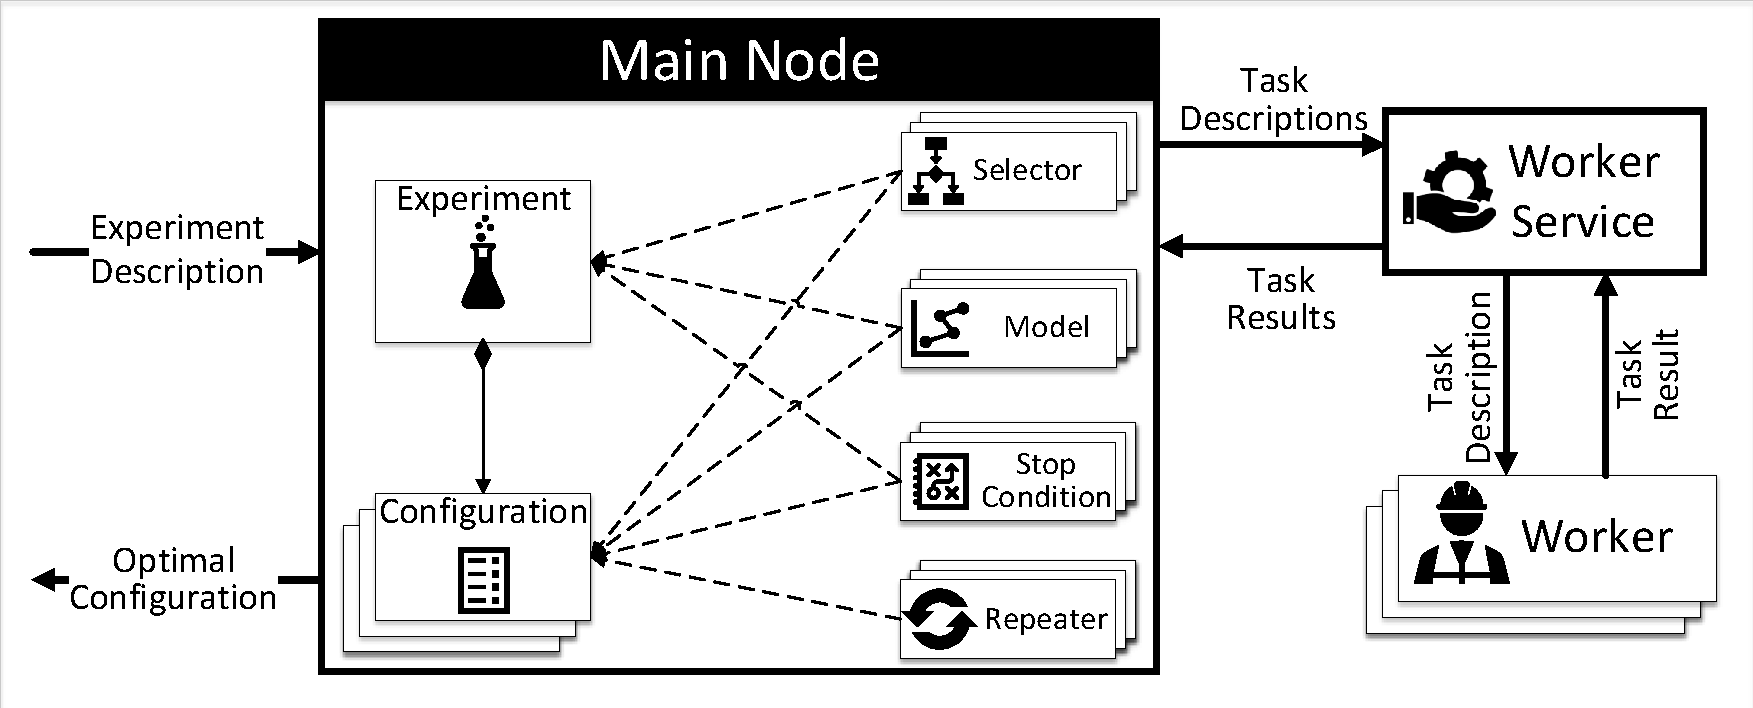
\includegraphics[width=\textwidth]{images/BRISEarch.pdf}
	\caption[The high-level architecture of BRISE]{The high-level architecture of BRISE}
	\label{fig:BRISEarch}
\end{figure}

Figure~\ref{fig:BRISEarch} shown the high-level architecture of BRISE.
Configurable part consist of 
	\paragraph{Experiment description} - describes the experiment, parameters that need to tune, the objective of the experiment, and expected values to detect outliers.
	\paragraph{Selector} - selection algorithm that is used to get the combination of parameters from the search space of all possible combinations. BRISE has two selection algorithms out of the box: Sobol sampling~\cite{sobol99} and Fedorov's exchange algorithm~\cite{fedorov13}. 
	\paragraph{Model} - predict new configuration. New Model builds after each iteration of measurement of configuration, and if Model predicts a valid result, this configuration goes to be measured in the next iteration. BRISE has several models out of the box.
	\paragraph{Stop condition} - the component that analyzes the results of the experiment, validates the result, and makes a decision to stop the experiment or continue. There are many different stop conditions that could work as a combination of criteria.
	\paragraph{Repeater} - component of BRISE that decide about the number of measurement for each configuration to get need accuracy of the results. 
	\paragraph{Worker} - contains the process that BRISE needs to tune. Run this process with different configurations and returns the metric of this configuration to use it in the next model build.
All components from the configurable part could be extended by users to achieve their goals.

BRISE has two modes: \textit{Search space exploration} and \textit{Hyperparameter tuning}.
First one is used to get information about search space of hyperparameters. In this mode there is no predictions cause BRISE uses the selector to cover the search space. As a result of using BRISE without predictions, the model component is disabled. Also stop condition is disabled in this mode and BRISE stops after it have covered all search space. Repeater works as it should to achieve needed accuracy.

The second mode is used to find the optimized values for hyperparameters. All components of the main node are used in this mode.

The main principle of how BRISE works in both modes is the same, but 
Search space exploration mode has one exception.

User prepare target system that will runing in workers and measure the result for specified configuration of hyperparameters.
After that user describe the experiment description - JSON file that contains all information about hyperparameters, their ranges and default values, result structure, expected ranges for result values and the max time needed to run one task.

The user input of BRISE is experiment description, that in BRISE transforms into Experiment object. After that BRISE start working.

It start with measurement of default configuration. When the default configuration had been measured, selector gives set of new configurations to be measured. After measurments workers return the results to main node. The repeater checks the result and decide to measure this configuration one more time or results has needed accuracy. 

On the next step model component tries to build the model and validate itself. If built model is valid then it predicts new configuration. if the model is not valid, BRISE get new configuration from the selector. BRISE send it to worker service to measure and get the result. If SPL working in Search space exploration mode, the model build step is skipped and new configuration always received from the selector. 

This measurements are performing until stop condition criteria in stop condition component are met.









